\section{Introduction}
	\subsection{Schr\"odinger formalism}
	
		\begin{equation}
			\hat{f}\Phi =  E \Phi
		\end{equation}
	
		\begin{equation}
			\Phi \rightarrow dP = |\Phi|^2dq
		\end{equation}
		
		\begin{equation}
			x \leftrightarrow \hat{x}
		\end{equation}

		\begin{equation}
			p_x \leftrightarrow -i\hbar \frac{\partial}{\partial x}
		\end{equation}
	
		\begin{equation}
			f \leftrightarrow \hat{f}
		\end{equation}	
		
		\begin{equation}
			\bar{f} = \int \hat{f}dp = \int \Phi^* \hat{f} \Phi dq 
		\end{equation}
		
		\begin{equation}
			[\hat{f}, \hat{g}] = \hat{f}\hat{g} - \hat{g}\hat{f}
		\end{equation}

		\begin{equation}
		\{\hat{f}, \hat{g}\} = \hat{f}\hat{g} + \hat{g}\hat{f}
		\end{equation}
	
	\subsection{Heisenberg formalism}
		\epigraph{Schr\"odinger was good at math, which is why his quantum mechanics formalism is full of complex mathematical constructs. Heisenberg, on the other hand, had a lot of difficulty with math, which is why his matrix quantum mechanics formalism is limited almost exclusively to linear algebra constructs}{Roman ... }
	
		\begin{tabular}{c | c | c }
			Name & Schr\"odinger & Heisenberg \\
			\hline
			\hline
			\ &&\\
			
			 State Basis & Wave function of basis states $ \{ \Phi_n \} $ & Column vector of basis states $\begin{pmatrix}\phi_1\\...\\ \phi_n\end{pmatrix}$ \\[3ex]		
			\hline
			\hline
			\ &&\\
			
			Observables & Operator $ \bar{f} = \int \Phi_n^* \hat{f} \Phi_m$ & Operator matrix $\begin{pmatrix}\phi_{11} & ... & \phi_{n1} \\ & ... & \\ \phi_{1n} & ... & \phi_{nn}\end{pmatrix}$ \\[3ex]
			\hline
			\hline
			
			\ &&\\
			Shr\"odinger Equation & $ \hat{f}\Phi =  E \Phi$ & $\begin{pmatrix}\phi_{11} & ... & \phi_{n1} \\ & ... & \\ \phi_{1n} & ... & \phi_{nn}\end{pmatrix} \begin{pmatrix}\psi_1\\...\\ \psi_n\end{pmatrix} = \lambda \begin{pmatrix}\psi_1\\...\\ \psi_n\end{pmatrix}$ \\[3ex]
			\hline
			\hline			
		\end{tabular}
	
		\subsubsection{Building an operator's matrix}
			For a system with a discrete state basis, $\{\Psi_n \}$, any state of the system can be described as a linear combination of the basis' wave functions:
			
			\begin{equation}
				\Psi = \sum_{n}a_n\Psi_n
			\end{equation}
			
			Observable $\bar{f}$  for such a wave function can be decomposed into a sum over the basis state wave functions:
			
			\begin{align}
				\bar{f} = & \int \Psi^* \hat{f} \Psi dq = \int \sum_{n}a_n^*\Psi_n^* \hat{f} \sum_{m}a_m\Psi_m dq \nonumber \\ 
				=  &\sum_{n}\sum_{m}a_n^* a_m \int \Psi_n^* \hat{f} \Psi_m dq = \sum_{n}\sum_{m}a_n^* a_m f_{nm}(t) \nonumber \\
				=  &\sum_{n}\sum_{m}a_n^* f_{nm}(t) a_m
			\end{align}
			
			Where $f_{nm}$ is the operator matrix.
			
			\subsubsection{$f_nm(t)$ time dependence}
				\hl{Move to appendix?}
				
				Solutions to the time-independent Shr\"odinger equation: 
				\begin{align}
					\hat{H}\Psi_n &= E_n \Psi_n \\
					\Psi_n(t) &= e^{-\frac{i}{\hbar}E_n t} \Phi_n
				\end{align}
				
				Which, in operator matrix terms translates into

				\begin{align}
					f_{nm}(t) &= \int \Psi_n^* \hat{f} \Psi_m dq = \int \Phi_n^* (e^{-\frac{i}{\hbar}E_n t})^* \hat{f} \Phi_m e^{-\frac{i}{\hbar}E_m t} dq \nonumber\\
					&=  e^{+\frac{i}{\hbar}E_n t}e^{-\frac{i}{\hbar}E_m t} \int \Phi_n^*\hat{f} \Phi_m  dq = e^{i \frac{E_n-E_m}{\hbar} t} \int \Phi_n^*\hat{f} \Phi_m  dq \nonumber\\
					&= f_{nm} e^{i \omega_{nm} t} 		
				\end{align}
				
			\subsubsection{Operator matrix properties}
				\begin{enumerate}
					\item The operator matrix is hermitian \footnote{$H^\dag = H = (H^*)^T$}
						Transposed operator:
						\begin{equation}
							(\int \Phi \hat{f} \Psi dq \quad)^T = \int \Psi (\hat{f})^T \Phi dq
						\end{equation}
						Complex conjugate:
						\begin{equation}
							(\hat{f})^* = \hat{f^*}
						\end{equation}	
						Hermitian conjugate:
						\begin{equation}
							\bar{f^*} = \int \Psi^* \hat{f}^\dag \Psi dq
						\end{equation}
						
						In operator matrix terms:
						\begin{align}
							(f_{nm}^*) &= \int \varphi_n^* \hat{f}^\dag \varphi_m dq = \int \varphi_n^* (\hat{f}^*)^T \varphi_m dq \nonumber \\
							&= \int \varphi_m (\hat{f}^* \varphi_n^*) dq = (\int \varphi_m^* \hat{f}^\dag \varphi_n dq )^* = (f_{mn})^*
						\end{align}
						Which means, if $f_{nm}$ is real, meaning $f_{nm}^* = f_{nm}$ that
						\begin{equation}
							f_{nm} = f_{mn}^* = f_{nm}^\dag
						\end{equation}
					\item The matrix' diagonal elements are time-independent and real
						\begin{equation}
							f_{nn} = \int \Psi_n \hat{f} \Psi_n dq \equiv \bar{f}_{n}
						\end{equation}
						
						Where $\bar{f}_{n}$ is the value of observable $f$ in basis state $n$.
						
					\item The matrix of the product of two operators is the product of their matrices
					
						For operators $\hat{f}$ and $\hat{g}$, what is the operator matrix for operator $\hat{f}\times\hat{g}$ ~--- $(\hat{f}\times\hat{g})_{nm}$?

						\hl{Move to appendix?}						
						\begin{align}
							\hat{f}\varphi_n &= \sum_m f_{mn} \varphi_m \\
							\int \varphi_k^* dq \times \hat{f}\varphi_n &=  \int \varphi_k^* dq \times \sum_m f_{mn} \varphi_m \nonumber \\
							\int \varphi_k^* \hat{f}\varphi_n dq &= \sum_m f_{mn} \int \varphi_k^* \varphi_m dq
							f_{kn} = \sum_m f_{mn} \delta_{km} = f_{kn}
						\end{align}
						Because for state basis ${\varphi_n}$, $\varphi_n$ and $\varphi_m$ are orthogonal for all $m \not= n$.
						
						Using 1.18, we can write:
						\begin{align}
							\hat{f}\hat{g}\varphi_n &= \hat{f}(\hat{g}\varphi_n) = \hat{f} \sum_k g_kn \varphi_k = \sum_k g_{kn} \hat{f} \varphi_k \nonumber \\
							&= \sum_k g_{kn} \sum_m f_{mk} \varphi_m = \sum_{k,m} g_{kn}f_{mk}\varphi_m \nonumber \\ 
							&= \sum_{k,m} f_{mk}g_{kn}\varphi_m
						\end{align}
						And knowing that:
						\begin{equation}
							(\hat{f}\hat{g})\varphi_n = \sum_m(\hat{f}\hat{g})_{nm}\varphi_m
						\end{equation}
						We end up with:
						\begin{equation}
							(\hat{f}\hat{g})_{mn} = \sum_k f_{mk}g_{kn}
							\label{fgproduct}
						\end{equation}
						
					\item The operator's matrix is equivalent to the operator
						\begin{equation}
							\Psi = \sum_m c_m \varphi_m
						\end{equation}
						
						\begin{align}
							\hat{f} \Psi &= f \Psi \\
							\hat{f}\sum_m c_m \varphi_m &= f\sum_m c_m \varphi_m \nonumber \\
							\int \varphi_n^* \hat{f}\sum_m c_m \varphi_m dq &=  \int \varphi_n^* f\sum_m c_m \varphi_m dq\nonumber \\
							\sum_m c_m \int \varphi_n^* \hat{f} \varphi_m dq &= f \sum_m c_m \int \varphi_n^* \varphi_m dq \nonumber \\
							\sum_m c_m f_{nm} &= f \sum_m c_m \delta_{nm} \nonumber \\
							\sum_m c_m f_{nm} &= f c_n \\							
						\end{align}
						
						\begin{align}
							\sum_m c_m f_{nm} &= f c_n \nonumber\\
							\sum_m f_{nm} - f \delta_{nm} c_m &= 0 \Rightarrow \nonumber\\
							\mid\mid f_{nm} - f\delta_{nm}\mid\mid &= 0 \\
						\end{align}
					
				\end{enumerate}
	
			\subsection{Switching to a different state basis}
				$\{\varphi_n(q) \}$ and $\{\varphi_n'(q) \}$ are two different basis's.
				
				\begin{align} 
					\varphi_n'(q) &= \sum_m S_{mn} \varphi_n(q) \\
					\varphi_n' &= \hat{S} \varphi_n 
				\end{align}
				
				Where $\hat{S}$ is the transition operator. If the new basis$\{\varphi_n^{'}(q) \}$ is orthogonal, meaning:
				
				\begin{equation}
					\int \varphi_m'^* \varphi_n' dq = \delta_{mn}
				\end{equation}
	
				then $\hat{S}^\dag = \hat{S}^{-1}$.
				\begin{align}
					\int \varphi_m'^* \varphi_n' dq &= \delta_{mn} \nonumber \\
					\int \hat{S}^*\varphi_m^*  \hat{S}\varphi_n dq &= \delta_{mn} \nonumber \\					
					\int \varphi_m^* (\hat{S}^*)^T \hat{S}\varphi_n dq &= \delta_{mn} \nonumber \\					
					\int \varphi_m^* \sum_l S_{ml}^* S_{ln}\varphi_n dq &= \delta_{mn} \nonumber \\				
					\sum_l S_{ml}^* S_{ln} \int \varphi_m^* \varphi_n dq &= \delta_{mn} \nonumber \\
					\delta_{mn}(\sum_l S_{ml}^* S_{ln} - 1) &= 0 \quad \Rightarrow \nonumber \\
					\hat{S}^\dag &= \hat{S}^{-1} \quad (S_{mn}^\dag = S_{nm}^*)
				\end{align}
				
				Operators in the new basis can be written as:
				\begin{align}
					\int \varphi_m'^* \hat{f} \varphi_n' dq &= \int(\hat{S}^* \varphi_m^* )(\hat{f} \hat{S} \varphi_n) dq = \nonumber \\
					= \int \varphi_m^* \hat{S}^{*T} \hat{f} \hat{S} \varphi_n) dq &= \int \varphi_m^* \hat{f}' \varphi_n dq \Rightarrow \nonumber \\
					\hat{f}' = \hat{S}^{*T}\hat{f}\hat{S} &= \hat{S}^\dag \hat{f} \hat{S} = \hat{S}^{-1}\hat{f}\hat{S}
				\end{align}
				
				\paragraph{The operator's matrix's trace} is the sum of the operator matrix's diagonal elements:
					\begin{equation}
						Sp \hat{f} = \sum_n f_{nn}
						\label{spf}
					\end{equation}
					
					\begin{enumerate}
						\item The trace of the product of two operators is invariant to the order of the operators 
							\begin{equation}
								Sp (\hat{f} \hat{g}) = Sp (\hat{g} \hat{f})
								\label{spfg}
							\end{equation}
							According to \ref{spf}, $Sp \hat{f} = \sum_n f_{nn}$, therefore (using \ref{fgproduct}):
							\begin{align}
								Sp (\hat{f}\hat{g}) &= \sum_n (\hat{f}\times \hat{g})_{nn} \nonumber \\	
								&= \sum_n \sum_k f_{nk} g_{kn} \quad\text{and}\\
								Sp (\hat{g}\hat{f}) &= \sum_n (\hat{g}\times \hat{f})_{nn} \nonumber \\	
								&= \sum_n \sum_k g_{nk} f_{kn}, \quad n\rightarrow k; k\rightarrow n\nonumber \\
								= \sum_k \sum_n g_{kn} f_{nk} &= \sum_n \sum_k f_{nk} g_{kn}
							\end{align}
						\item The trace of the product of three or more operators is invariant to the cyclic permutation of the operators
							\begin{equation}
								Sp (\hat{f} \hat{g} \hat{h}) = Sp (\hat{h} \hat{f} \hat{g}) = Sp (\hat{g} \hat{h} \hat{f})
								\label{spfgh}
							\end{equation}
							According to \ref{spfg}
							\begin{align}
								Sp(\hat{f}(\hat{g}\hat{h})) &= Sp((\hat{g}\hat{h})\hat{f}) \quad\text{and} \\
								Sp((\hat{f}\hat{g})\hat{h}) &= Sp(\hat{h}(\hat{f}\hat{g})) 
							\end{align} 
							Which is equivalent to \ref{spfgh} because matrix multiplication is associative.
					\end{enumerate}
	
					The operator's matrix's trace is invariant to the basis.
					\begin{equation}
						Sp \hat{f}' = Sp \hat{S}^{-1}\hat{f}\hat{S}  = Sp \hat{S}\hat{S}^{-1}\hat{f} =  Sp \hat{f} 
					\end{equation}
				\paragraph{Commutators}
					Two operators commute if and only if they share a set of basis states. Or, in other words, there exist as basis in which they are both diagonal.
					
					If $\hat{f}$ and $\hat{g}$ commute, then:
					\begin{equation}
						[\hat{f}, \hat{g}] = \hat{f}\hat{g} - \hat{g}\hat{f} = 0
					\end{equation}
					Which means that	
					\begin{equation}
						\sum_k f_{mk}g_{kn} = \sum_k  g_{mk}f_{kn}
					\end{equation}
					If $\{\varphi_n\}$ are eigenfunctions of $\hat{f}$, then $f_{nm} \not= 0$ only if $n=m$ $\rightarrow$
					\begin{align}
						f_{mm}g_{mn} &= g_{mn} f_{nn} \nonumber \\
						g_{mn} (f_{mm} - f_{nn}) &= 0
					\end{align}
					Meaning that $g_{mn} = 0$ if $m \not= n$ 
				
	\subsection{Pauli uncertainty principle}
		The Pauli uncertainty principle states that if the operators of two observables do not commute, than we cannot measure both observables with arbitrary precision at the same time. In other words, that to more certain are we about one observable, the more uncertain we are about the other. For example:
		\begin{align}
			[\hat{x}, \hat{p_x}] = i\hbar \\
			\Delta x \Delta p_x \geq \hbar
		\end{align} 
		
		or, for an exact relation,
		\begin{align}
			\sigma_{x} \sigma_{p_x} &\geq \frac{\hbar}{2}\\
			\sigma_{x} = \sqrt{<\Delta x^2>}&\quad 
			\sigma_{p_x} = \sqrt{<\Delta p_x^2>} \\
		\end{align}
		
		
		\subsubsection{Single-slit electron diffraction}
			\begin{figure}[!h]
				\centering
				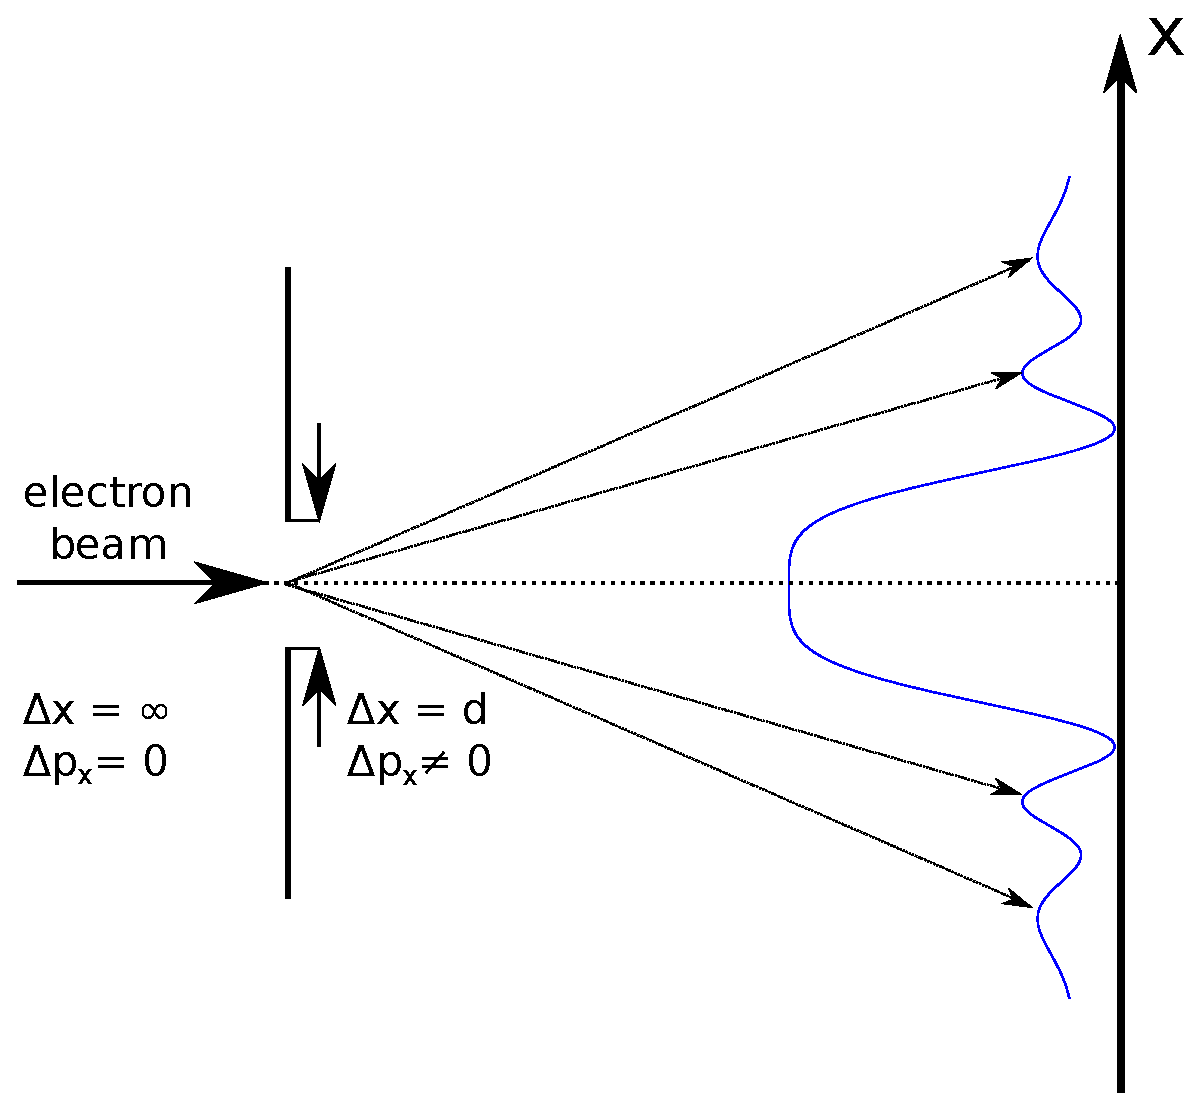
\includegraphics[width=0.45\textwidth]{./figs/ElectronDiffraction.eps}
				\caption{Single-slit electron diffraction}
				\label{electrondiffrac}
			\end{figure}
			
			\begin{align}
				b \sin(\theta) = \lambda \\
				\Delta p_x = p \sin(\theta) \\
				\Delta x = d
			\end{align}
			Using the relation for the de Broglie wavelength
			\begin{equation}
				\lambda = \frac{h}{p} = \frac{2*\pi *\hbar}{p}
			\end{equation}
			We get, considering
			\begin{equation}
				\Delta x \Delta p_x = d \sin(\theta) \frac{2\pi\hbar}{\lambda} = 2 \pi \hbar
			\end{equation}
			\begin{equation}
				\Delta x \Delta p_x \approx \hbar
			\end{equation}
			
		\subsubsection{Black holes}
			\epigraph{And now let's talk about black holes}{Ivan Iorsh}
			For an average star we can say that it's electrically neutral, has about the name number of protons as neutrons and is approximately spherical:
			\begin{align}
				\bar{e} \rightarrow N \\
				\bar{p} \rightarrow N \\
				\bar{n_0} \rightarrow N \\
				V = \frac{4}{3}\pi R^3 \\
				M_{\astrosun} = 2 m_p N
			\end{align}
			\begin{figure}[!h]
				\centering
				%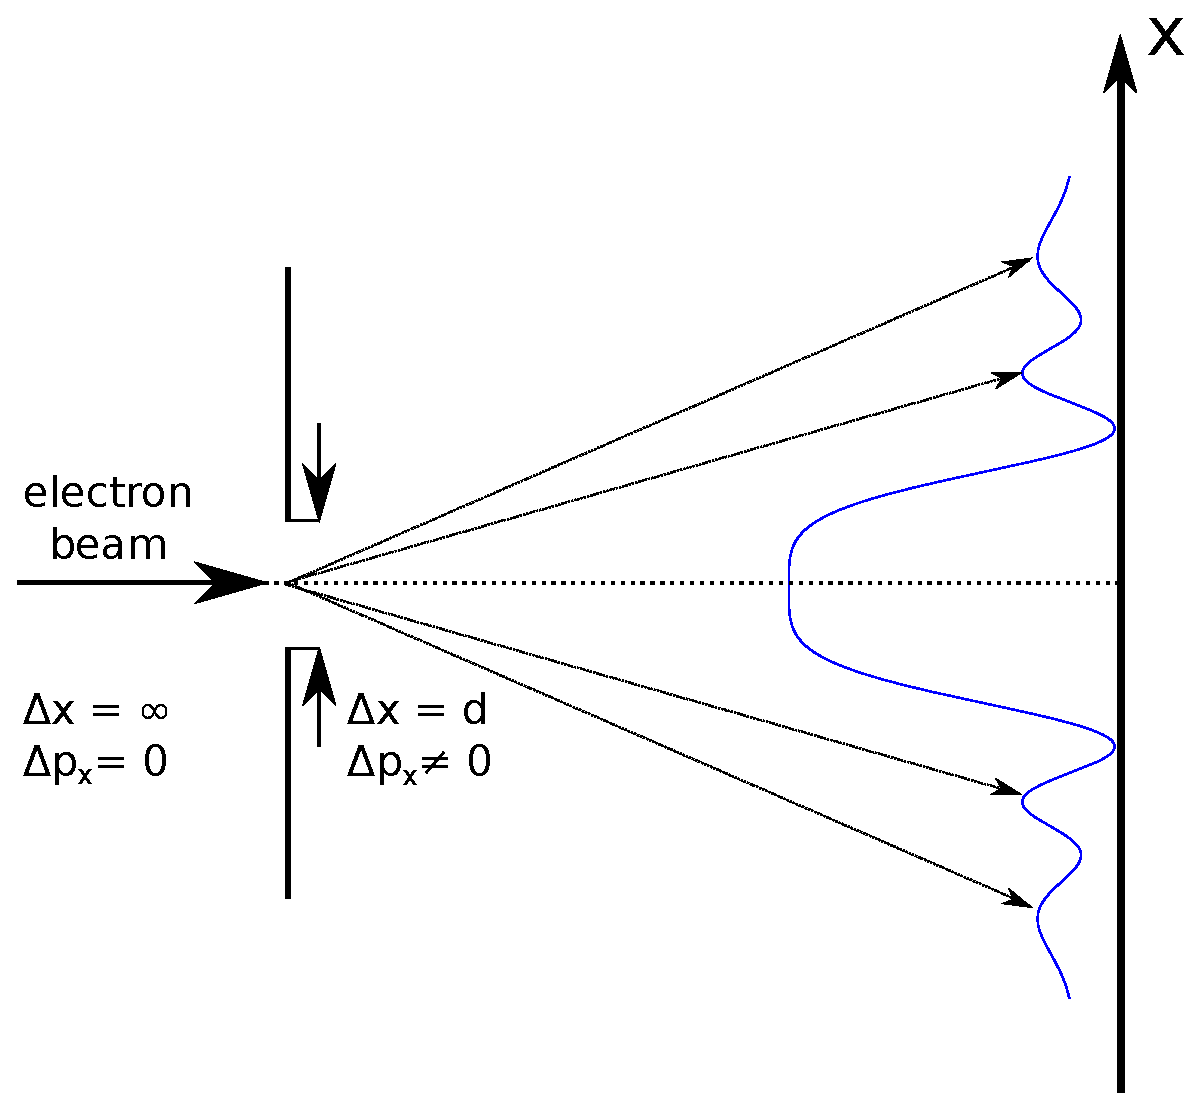
\includegraphics[width=0.45\textwidth]{./figs/ElectronDiffraction.eps}
				\caption{Spherical horse in a vacuum}
				\label{star}
			\end{figure}
			Knowing the total volume we can estimate the average volume occupied by each electron, $d_e$:
			\begin{equation}
				d_e = \left( \frac{\frac{4}{3}\pi R^3}{N} \right) ^{\frac{1}{3}} = \frac{R}{N^{\frac{1}{3}}}\left( \frac{4}{3}\pi \right)^{\frac{1}{3}}
			\end{equation}
			\hl{TODO: MOVE TO END:}
			Average electron position, taking into account the fact that the electrons are confined:
			\begin{equation}
				\langle \Delta d^2 \rangle = \langle d^2 \rangle + \cancelto{0}{\langle\Delta d \rangle^2} =  \langle d^2 \rangle
			\end{equation}
			And considering that electron positions $d$ are of the same order as their \hl{dispersion} $\Delta d \approx d$; and the same for their momentum, $\Delta p \approx p$ the Pauli uncertainty principle can be written as (for one electron):
			\begin{align}
				\Delta p \Delta d \gtrsim \frac{\hbar}{2}; \qquad v \frac{p}{m_e} \\
				\Delta p \approx = \frac{\hbar}{2 \Delta d} = \frac{\hbar}{2 d} \\
				E_{kinetic} = \frac{m_ev^2}{2} = \frac{p^2}{2m_e} = \frac{\hbar^2}{8d^2m_e}
			\end{align}
			And for $N$ electrons:
			\begin{equation}
				E_{kN} = \frac{N\hbar^2}{8d^2m_e}
			\end{equation}
			For an average star,
			\begin{align}
				M_{\astrosun} \approx& 2*10^{33} \si{g} \\
				R_{\astrosun} \approx& 6*10^5 \si{m} \\
				m_p \approx& 10^{-27} \si{kg} \\
				m_e \approx& 10^{-30} \si{kg} \\
				\hbar =& 1.05 * 10^{-34} \si{J * s}
			\end{align}
			The average speed of an electron in the star is\hl{Explicit calc}
			\begin{align}
				V =& \frac{p}{m_e} = \frac{\hbar}{m_e} \frac{N^{\frac{1}{3}}}{R}\left(\frac{4}{3}\pi\right)^{-\frac{1}{3}} = \frac{\hbar}{m_e} \left( \frac{M}{2m_p}\right)^{\frac{1}{3}}\frac{1}{R}\left(\frac{4}{3}\pi\right)^{-\frac{1}{3}} =\\
				=& \qquad \text{...} \\
				\approx& 10^8 \si{\frac{m}{s}} \hl{\approx \frac{1}{3}c}
			\end{align}
			Which is highly relativistic. 
		\subsubsection{Quantum Pencil}
			\cite{easton2007quantum}
		
	\subsection{Problems}